\chapter{緒論}
\label{chapter:intro}


\section{5G 概觀}
\label{sec:5g_intro}

行動網路的發展至今,以然數十年有餘,概約每十年變換進行一次跳躍性的革新。從最初的 1G 與 2G,著重於語音的通訊,並企圖達到移動通訊的能力,讓人們可以隨時隨地的互相通訊。進入了 3G 的時代後,行動網路加入了封包交換 (packet switching) 的能力,使得網際網路透過手機與行動網路進入大眾的手上。隨著智慧型手機的普及,透過手機與網路接觸的使用體驗大幅增加,人類對行動網路頻寬的需求日益不足,4G 的出現便是為了彌補這樣的需求,從此人們得以享有穩定的行動網路服務。

縱觀 1G 到 4G 的演進,行動網路再再為了滿足人類的使用而眼進。然而到了 5G 的時代,行動網路卻以不再僅僅侷限於個人用戶的需求,而是企圖符合更多的使用場景,達到「萬物聯網」的野心。為滿足如此龐大的野心,過往的架構將不再適用於此,因此有了 5G 的出現。

\begin{figure}[htbp]
    \centering
    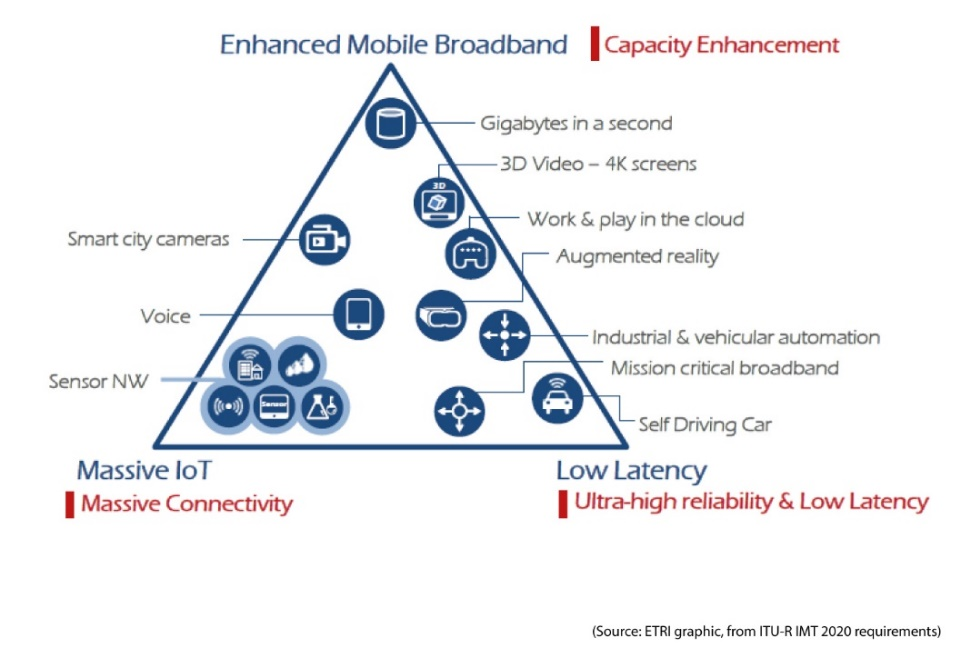
\includegraphics[height=!,width=0.8\linewidth,keepaspectratio=true]{figures/usage_scenarios_of_IMT_for_2020}
    % [] 放的是顯示在 list of figure 的文字
    % {} 放的是顯示在圖下方的文字
    \caption[行動網路 2020 及未來之應用場景]{{\footnotesize 行動網路 2020 及未來之應用場景~\cite{IMT_2020}}}
    \label{fig:IMT_2020}
\end{figure}

5G 全名為第五代行動通訊網路,系指繼 4G 之後由 3GPP 組織所定義出的最新行動網路通訊技術,為滿足更多種類的情景與應用,國際行動通訊組織 (International Mobile Telecommunications, IMT) 於國際電信聯盟無線通訊部門 (International Telecommunication Union Radiocommunication Sector, ITU-R) 制定 IMT-2020~\cite{IMT_2020},希望以技術的角度,提出 5G 網路的三大願景:
\begin{enumerate*}
\item 增強行動寬頻通訊 (enhanced Mobile Broadband, eMBB):指希望增強行動網路的頻寬,達到理論值 $20 Gbps$ 下行與 $10 Gbps$ 的上行,用以符合逐漸增加的 AR/VR 應用、4K/8K 影像串流等。
\item 超高可靠度低延遲通訊 (Ultra-Reliable and Low Latency Communications, URLLC):提供低於 $10^{-5}$ 的網路傳輸錯誤率,與低於 $1 ms$ 網路延遲服務品質,支援如遠端醫療、車聯網、高精密工業加工等應用。
\item 大規模物聯網通訊 (massive Machine Type Communications, mMTC):預期需服務超過 $10^{6}$ 個裝置同時連線上網的需求,使未來 IoT、工業 4.0 的場景可支援超高密集連線通訊。
\end{enumerate*}

為因應如此多元且靈活的網路特性,過往 4G 的專用網路架構以然不再適合,如何設計出得以適應如此多場景應用的網路架構,便是未來 5G 所要面臨的挑戰。

\section{研究動機與貢獻}
\label{sec:motivation_and_contribution}
% 動機
% 軟體化、虛擬化
% 現行網路是否真的符合三大特性
% 5G 仍有許多 4G 的影子,是否會成為突破的瓶頸
% CP 與 UP 的 msg 會日益增加
隨著 5G 的發展,為符合電信商與專有網路需求,行動網路也逐漸向 cloud-native 的趨勢靠攏。就由網路功能虛擬化 (virtualization)、軟體化 (softwarization),網路功能可以以軟體甚至是容器的方式進行佈署,大大提高行動網路佈署上的擴展性 (scalability)。但是有別於 4G 專業設備的佈署方式,以軟體形式佈署勢必無法達到硬體加速的效能,如此一來將如何達到增強彭寬的效果?另外目前 (R15) 的 5G 網路架構並未能滿足低延遲的需求,尤其在 NF 與 SBI 的設計之下,控制層反而需要通過比以往 4G 更多的分工處理才能完成,且雖然在網路功能結構上有所改變,但在流程上還是可以看到大量的 4G 流程的影子,這樣的設計能否因應未來應用上劇烈的挑戰?最後,隨著更多元的設備連接,控制層訊號的數量將遠超以往,該如何解決控制層通訊延遲與壅塞的狀況?
% 貢獻
% 藉由 DPDK 與 SM 加速通訊效率
% 最佳化 HO 流程
% 提供 NFV, cloud native 方案, reliablity & scalibility
% 測試基於 OpenNetVM 的 AMF, SMF, 與 UPF 的效能
本篇論文針對上訴的問題,提出了以下幾點改變與嘗試:

\begin{itemize}
\item 我們利用具有彈性及擴展性的網路功能虛擬化 (Network Function Virtualization, NFV) 平臺,設計了於同一節點上更有效率的核心網路溝通方式。
\item 透過 DPDK 與共享記憶體的框架,重新設計與實作 SBI 與 N4 界面。透過共享記憶體,提供零記憶體複製 (zero-copy) 的節點內控制訊號通訊方式以減少訊號延遲,並藉由 DPDK 提供跨節點高流量的用戶端轉發。
\item 我們重新審視 3GPP 的流程,發現在換手流程上有不必要行為造成用戶端路徑增加,同時我們也提出了修改方法。
\end{itemize}

總結而言,本篇論文提出並實作了提高流量並降低延遲的 5G 核心網路架構。
